\documentclass[a4paper, 12pt]{article}

\usepackage{amsmath} %Todos los paquetes de matematicas
\usepackage{amsthm}
\usepackage{mathtools}
\providecommand{\abs}[1]{\lvert#1\rvert}
\providecommand{\norm}[1]{\lVert#1\rVert}
\usepackage{yhmath}
\usepackage[utf8]{inputenc}
\usepackage[spanish]{babel}
\usepackage{wrapfig} %Figuras flotantes
\usepackage{parselines}
\usepackage{enumitem}
\usepackage{xcolor}
\usepackage{graphicx}
\graphicspath{{images/}}
\usepackage{subcaption}
\usepackage[left=2cm,right=2cm,top=2cm,bottom=2cm]{geometry}
\usepackage{eurosym} %Euro, de nada misniños

\theoremstyle{definition}
\newtheorem{ej}{Ejercicio}



\title{\textbf{Relación de ejercicios 2 EDIP}}
\author{Carlos García, Bora Goker, Javier Gómez,  \\ Ana Graciani, J.Alberto Hoces}
\date{2020/2021}

\setlength{\parindent}{0px}

\begin{document}

\maketitle

\begin{ej}
En una encuesta de familias sobre el número de individuos que la componen \((X)\) y el número de personas activas en ellas \((Y)\) se han obtenido los siguientes resultados:
\begin{center}
\begin{tabular}{c|cccc}
	\(X/Y\) & 1 & 2 & 3 & 4 \\
	\hline
	1 & 7 & 0 & 0 & 0 \\
	2 & 10 & 2 & 0 & 0 \\
	3 & 11 & 5 & 1 & 0 \\
	4 & 10 & 6 & 6 & 0 \\
	5 & 8 & 6 & 4 & 2 \\
	6 & 1 & 2 & 3 & 1 \\
	7 & 1 & 0 & 0 & 1 \\
	8 & 0 & 0 & 1 & 1
\end{tabular}
\end{center}

\begin{enumerate}[label=\alph*)]
	\item Calcular la recta de regresión de \(Y\) sobre \(X\).
	\begin{center}
	\begin{tabular}{c|c c c c c c c}
	\(X/Y\) & 1 & 2 & 3 & 4 & \(n_{i.}\) & \(n_{i.}x_i\) & \(n_{i.}x_i^2\) \\
	\hline
	1 & 7 & 0 & 0 & 0 & 7 & 7 & 7 \\
	2 & 10 & 2 & 0 & 0 & 12 & 24 & 48 \\
	3 & 11 & 5 & 1 & 0 & 17 & 51 & 153 \\
	4 & 10 & 6 & 6 & 0 & 22 & 88 & 352 \\
	5 & 8 & 6 & 4 & 2 & 20 & 100 & 500 \\
	6 & 1 & 2 & 3 & 1 & 7 & 43 & 252 \\
	7 & 1 & 0 & 0 & 1 & 2 & 14 & 98 \\
	8 & 0 & 0 & 1 & 1 & 2 & 16 & 128 \\
	\(n_{.j}\) & 48 & 21 & 15 & 5 & 89 \\
	\(n_{.j} y_j\) & 48 & 42 & 45 & 20 \\
	\(n_{.j} y_j^2\) & 48 & 84 & 135 & 80 
	\end{tabular}
	\end{center}
	
La recta de regresión lineal de \(Y\) sobre \(X\) viene dada por la expresión:
\[
	y - \overline{y}  =\frac{\sigma_{xy}}{\sigma_x^2} (x - \overline{x}) \Rightarrow y = \frac{\sigma_{xy}}{\sigma_x^2}x - \frac{\sigma_{xy}}{\sigma_x^2} \overline{x} + \overline{y}
\]
Por lo tanto, comencemos calculando las medias aritméticas y la varianza de \(x\) y la covarianza:
\[
	\overline{x} = \frac{1}{n} \sum_{i=1}^{8} x_i n_{i.} = 3.8427 \text{ individuos} \qquad \overline{y} = \frac{1}{n} \sum_{j=1}^{4} y_j n_{.j} = 1.7416 \text{ personas activas}
\]
\[
	\sigma_x^2 = \frac{1}{n} \sum_{i=1}^{8} n_{i.} x_i^2 - \overline{x}^2 = 2.5146 \text{ individuos}^2
\]
\[
	\sigma_{xy} = \frac{1}{n} \sum_{i=1}^{8} \sum_{j=1}^{4} n_{ij} x_i y_j - \overline{x}\ \overline{y} = 0.7907
\]
Por lo tanto, la recta de regresión de \(Y\) sobre \(X\) quedaría:
\[
	y = \frac{\sigma_{xy}}{\sigma_x^2}x - \frac{\sigma_{xy}}{\sigma_x^2} \overline{x} + \overline{y} = 0.3144x + 0.5333
\]

	\item ¿Es adecuado suponer una relación lineal para explicar el comportamiento de \(Y\) a partir de \(X\)?
	
Para ver cómo de adecuado es suponer dicha relación calculamos el coeficiente de correlación lineal:
\[
	r^2 = \sqrt{\frac{\sigma_{xy}^2}{\sigma_x^2 \sigma_y^2}} \qquad r = \sqrt{r^2}
\]
Ahora calculamos la varianza de \(Y\):
\[
	\sigma_y^2 = \frac{1}{n} \sum_{j=1}^{4} n_{.j} y_j^2 - \overline{y}^2 = 0.8657 \text{ personas activas}^2
\]
Por tanto:
\[
	r^2 = \frac{0.7907^2}{2.5146 \cdot 0.8657} = 0.2872 \qquad r = 0.536
\]
Observando estos resultados podemos afirmar que no es adecuado suponer esta relación linear puesto que el coeficiente de correlación lienal está demasiado alejado de 1.

\begin{figure}[h!]
	\centering
	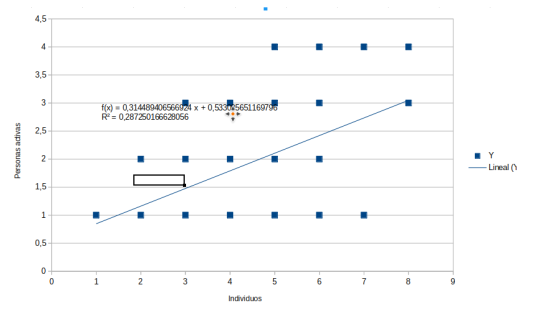
\includegraphics[scale=0.55]{images/ejer3.png}
\end{figure}

\end{enumerate}

\end{ej}

\end{document}